\livelloA{Methodology}

\begin{frame}
  \begin{scriptsize}
    Statistics can be divided in three areas:
    \vspace{.25cm}
    \begin{description}
      \item [I] DESCRIPTIVE STATISTICS
      \begin{description}
        \item [a)] Presentation of data in tables and graphs.
        \item [b)] Synthetic indices that describe the distribution of data.
      \end{description}
      \vspace{.25cm}
      \item [II] MATHEMATICAL STATISTICS
      \begin{description}
        \item [] Probability calculus and theoretical distributions. \\
          Theoretical probability distributions: Binomial, Poisson, Hypergeometric, Normal, ...
      \end{description}
      \vspace{.25cm}
      \item [III] INFERENTIAL STATISTICS
      \begin{description}
        \item []\textit{Deduction of general laws from a random sample of data}.
        \item [a)] Parametric hypothesis (about mean, variance, $\dots$) and functional hypothesis (about the distribution).
        \item [b)] Univariate, bivariate, multivariate distributions.
        \item [c)] Parametric and non-parametric statistics.
        \item [d)] One-sample, two-sample, $n$-sample tests.
      \end{description}
    \end{description}
  \end{scriptsize}
\end{frame}



\livelloA{Data type and scale of measure}

\begin{frame}
  \vspace*{.75cm}
  During the statistical analysis, data features have to be considered carefully. \\
  \vspace*{.75cm}
  The experimental phase in which information are collected is a key point: both description methods and applicable tests rely on experimental phase. \\
\end{frame}

%%%%%%%%%%%%%%%%%%%%%%%%%%%%%%%%%%%%%%%%%
\begin{frame}
\begin{center}
\textbf{Statistical universe}
\end{center}

\vspace {0.5cm}
\onslide<1>{
\begin{tiny}
	\begin{tikzpicture}[level distance=12mm] % la distanza tra i blocchi in altezza
	\tikzstyle{level 1}=[sibling distance=60mm]
                \tikzstyle{every node}=[fill=blocco!50,rounded corners,text width=1.3cm, text height=0.3cm] % la lunghezza dei blocchi
                \tikzstyle{edge from parent}=[blocco,thick,draw]
	 	\tikzstyle{level 2}=[sibling distance=32mm] % la distanza tra i blocchi in larghezza
                  \node(A1)[ text width=3cm] [fill=blocco]{Statistical data}
			child {node(B1) {\textbf{Continuous}}
%				child {node (C1) {\textbf{Nominal }}}
%				child {node (C2) {\textbf{Ordinal }}}
			}
			child {node(B2) {\textbf{Discrete}}
				child {node  (C3) {\textbf{Quantitative}}}
				child {node  (C4){\textbf{Qualitative}}}
					child {node (D1) {\textbf{Nominal }}}
					child {node (D2) {\textbf{Ordinal }}}
			}
;


\path
 (A1)
  edge node[below=1mm,left=-23mm,fill=white]{\footnotesize}
 (B1);
\path
 (A1)
  edge node[below=3.2mm,left=-40mm,fill=white]{\footnotesize }
 (B2);

\path
 (B2)
  edge node[below=-3.2mm,left=5mm,fill=white,text width=0.6cm, text height=0.1cm]{\tiny  }
 (C3);

\path
 (B2)
  edge node[below=3.2mm,left=-5mm,fill=white,text width=0.6cm, text height=0.1cm]{\tiny  }
 (C4);


\path
(C4)
 edge node[below=-8mm,left=10mm,fill=white,text width=0.6cm, text height=0.1cm]{\tiny  }
(D1);



\path
(C4)
 edge node[below=-3.2mm,left=10mm,fill=white,text width=0.6cm, text height=0.1cm]{\tiny  }
(D2);


         \end{tikzpicture}
\end{tiny}
}
\\
  \vspace{.35cm}
    Then, four types of scale exist:
    \begin{itemize}
	\item Continuous
	\item Discrete Qualitative Nominal
	\item Discrete Quantitative Ordinal
	\item Discrete Quantitative
  \end{itemize}

\end{frame}

%%%%%%%%%%%%%%%%%%%%%%%%%%%%%%%%%%%%%%%%%

\begin{frame}
  \vspace*{.15cm}
  Depending on the kind of data, different statistical options are available.\\
  \vspace*{.35cm}
  In general, on Qualitative data fewer statistical options are available than on quantitative data.\\
  \vspace*{.35cm}
  For example, on Quantitative data one might calculate the average, whereas, on qualitative nominal data this couldn't be done.\\ %% rivedere la forma dell'inglese di tutta la slide
  \vspace*{.35cm}
  Again, on Nominal data fewer statistical options are available than on Ordinal data.\\
  \vspace*{.35cm}
  Ordinal data can be treated as Nominal; the converse is not true.\\
  \vspace*{.35cm}
  Quantitative data can be always considered as Ordinal; the converse is not true.\\
\end{frame}

\begin{frame}
  \vspace{1.25cm}
  A \textbf{random variable} (or \textbf{stochastic variable}) is a variable whose values are associated to a probability law.\\
  \vspace{0.75cm}
  When a variable is not associated to a probability law it is called deterministic variable. \\
\end{frame}

\begin{frame}
  \vspace*{.25cm}
  The \textbf{random variables} are split into two main categories that are treated in different ways:
  \vspace*{.25cm}
  \begin{enumerate}
    \item \textbf{Discrete random variables} \\
    that are usually used to model qualitative (nominal or ordinal) data frequencies.
%     \begin{description}
%       \item[a.] \textbf{Quantitative discrete random variables}, that count the number of occurrences of an event, through \textbf{non-negative integers};
%       \vspace*{.15cm}
%       \item[b.] \textbf{Qualitative discrete random variables}, that can be further split into \textbf{nominal} or \textbf{ordinal} random variables.
%     \end{description}
    \vspace*{.25cm}
    \item \textbf{Continuous random variables} \\
      expressed on a continuous scale of values. Values are often associated to a proper \textbf{unit of measurement}.\\
  \end{enumerate}
\end{frame}

\begin{frame}
  The difference between \textbf{discrete} and \textbf{continuous} random variables is often not clearly defined, but it can depend from the number of \textbf{categories} associated to the variable.\\
  \begin{footnotesize}
    For example, the measurement of an height might be modeled by a discrete variable if it is measured in inches. If more decimal digits are considered then the number of categories increase and the same variable can be considered as a continuous variable.\\
  \end{footnotesize}
  \vspace*{.25cm}
  Discrete variables have less explicative power than continuous ones:\\
 \begin{itemize}
    \vspace*{-.25cm}
    \item statistics computed on continuous variables contains more information;
    \vspace*{-.15cm}
    \item to get good quality statistics using discrete variables a greater \textbf{number of observations} is required.
  \end{itemize}
  \vspace*{-.25cm}
  \begin{footnotesize}
    Data should be collected using the more accurate scale. When possible, data should be collected on a continuos scale. During the analysis data can be split into classes. This produce more readable results at the cost of information loss. \\
  \end{footnotesize}
\end{frame}



\livelloA{Classification tables}

\begin{frame}
  \vspace*{.75cm}
  \begin{small}
    \textbf{A set of observed data on a variable is called \textbf{Sample}.} \\
    \vspace*{.5cm}
    A first and basic data series processing is the \textbf{data ordering}, in ascending or descending way.\\
    \vspace*{.5cm}
    The difference between the highest value (maximum) and the lowest value (minimum) is called \textbf{range}.\\
    \vspace*{.5cm}
    Data can then be categorized into classes. The number of values (or \textbf{statistical units}) for each class can so be counted.\\
    \vspace*{.5cm}
    Values of frequencies of each category produce a \textbf{frequency distribution}, often called simply \textbf{distribution}.\\
  \end{small}
\end{frame}

\begin{frame}
  The table below reports the number of events counted on 45 time frames of the same length.
  \vspace*{.25cm}
  \begin{center}
    \begin{tabular}{|*{15}{c|}}
      \hline
      5 & 6 & 3 & 4 & 7 & 2 & 3 & 2 & 3 & 2 & 6 & 4 & 3 & 9 & 3 \\
      \hline
      2 & 0 & 3 & 3 & 4 & 6 & 5 & 4 & 2 & 3 & 6 & 7 & 3 & 4 & 2 \\
      \hline
      5 & 1 & 3 & 4 & 3 & 7 & 0 & 2 & 1 & 3 & 1 & 5 & 0 & 4 & 5 \\
      \hline
    \end{tabular}\\
    \vspace*{.2cm}
    \begin{scriptsize}
      \textbf{Tabella 1}: Number of events.
    \end{scriptsize}
  \end{center}
  The first step is the \textbf{definition of classes}:
  \vspace*{.25cm}
  \begin{itemize}
    \item the \textbf{minimum} (\textbf{0}, in the table) and the maximum (\textbf{9}) must be identified;
    \vspace*{.25cm}
    \item the number of data within each class\\ \small (how many zeros, how many ones, \dots) must be counted.
  \end{itemize}
\end{frame}

\begin{frame}
  \begin{table}
    \centering
    \begin{tiny}
      \begin{tabular}{|*{12}{c|}}
        \hline
        \textbf{Class} & \textbf{h} & \textbf{0} & \textbf{1} & \textbf{2} & \textbf{3} & \textbf{4} & \textbf{5} & \textbf{6} & \textbf{7} & \textbf{8} & \textbf{9}  \\
        \hline
        Absolute Freq & n & 3 & 3 & 7 & 12 & 7 & 5 & 4 & 3 & 0 & 1  \\
        \hline
        Relative Freq & f & 0.07 & 0.07 & 0.15 & 0.27 & 0.15 & 0.11 & 0.09 & 0.07 & 0.00 & 0.02 \\
        \hline
        Cumulative Abs Freq &  & 3 & 6 & 13 & 25 & 32 & 37 & 41 & 44 & 44 & 45  \\
        \hline
        Cumulative Rel Freq & F & 0.07 & 0.14 & 0.29 & 0.56 & 0.71 & 0.82 & 0.91 & 0.98 & 0.98 & 1.00  \\
        \hline
      \end{tabular}\\
      \vspace*{.2cm}
      \textbf{Table 2}: Distribution of absolute and relative frequencies of the number of events.\\
    \end{tiny}
  \end{table}
  \begin{footnotesize}
    \vspace*{-.2cm}
    The \textbf{class} row represents a category and, in this case, it is a count value. \\
    \vspace*{.2cm}
    The \textbf{absolute frequency} of a class is the count of data values of that class.\\
    \vspace*{.2cm}
    The \textbf{relative frequency} of a class is its absolute frequency divided by the total count of observations (in this example: 45).\\
    \vspace*{.2cm}
    The \textbf{cumulative (absolute or relative) frequency} of a class is the (absolute or relative) frequency of this class added to the sum of frequencies of all the lower classes. It requires data that can be ordered.
  \end{footnotesize}
\end{frame}

\begin{frame}
  \vspace*{.25cm}
  The use of the relative frequencies instead of absolute frequencies is especially useful when two or more distributions with different total counts of observation must be compared. \\
  \vspace*{.25cm}
  The cumulative frequency provides useful information to estimate the total count of observations less (or higher) than a set value. \\
  \vspace*{.25cm}
  \textbf{The frequency distribution provides an easy reading of most important characteristics of data:} in the example, the value 3 represents the \textbf{central tendency}. \\
  \vspace*{.25cm}
  The minimum and the maximum are, respectively, 0 and 9 and they provide the range, a measure of the \textbf{variability}.
\end{frame}

\begin{frame}
  \vspace*{.25cm}
  In this example, frequencies tend to decrease in a similar way in both directions starting from 3.
  As the number of classes with non null frequency above the center is greater than the number of classes below the center, the \textbf{shape} of the distribution is not symmetric but asymmetric.
  \vspace*{.5cm}
  \begin{table}
    \centering
    \begin{tiny}
      \begin{tabular}{|*{12}{c|}}
        \hline
        \textbf{Group} & \textbf{h} & \textbf{0} & \textbf{1} & \textbf{2} & \textbf{3} & \textbf{4} & \textbf{5} & \textbf{6} & \textbf{7} & \textbf{8} & \textbf{9}  \\
        \hline
        Absolute Freq & n & 3 & 3 & 7 & 12 & 7 & 5 & 4 & 3 & 0 & 1  \\
        \hline
        Relative Freq & f & 0.07 & 0.07 & 0.15 & 0.27 & 0.15 & 0.11 & 0.09 & 0.07 & 0.00 & 0.02 \\
        \hline
        Cumulative Abs Freq &  & 3 & 6 & 13 & 25 & 32 & 37 & 41 & 44 & 44 & 45  \\
        \hline
        Cumulative Rel Freq & F & 0.07 & 0.14 & 0.29 & 0.56 & 0.71 & 0.82 & 0.91 & 0.98 & 0.98 & 1.00  \\
        \hline
      \end{tabular} \\
    \vspace*{.2cm}
    \textbf{Table 3}: Distribution of absolute and relative frequencies of the number of events.\\
    \end{tiny}
  \end{table}
\end{frame}

\begin{frame}
  \vspace*{.5cm}
  \textbf{How many classes should be created when building a frequency table?} This is the first question when data grouping is required. The choice depends a lot on the total number \textbf{N} of observations and, to a lesser degree, data variability.\\
  \vspace*{.75cm}
  Frequency distributions tend to be representative of the phenomenon only when enough observations are available.\\
  \vspace*{.75cm}
  An empirical rule suggests to use 4-5 classes when observations are 10-15 until a maximum of 15-20 classes when observations are more than a hundred.\\
\end{frame}

\begin{frame}
  \begin{columns}
    \begin{column}{6cm}
      \textbf{Too few classes} cause a loss of information about distribution features. \\
    \end{column}
    \begin{column}{6cm}
      On the other side, \textbf{too many classes} return useless information because the distribution shape is not clearly visible.\\
    \end{column}
  \end{columns}
  \vspace{1.5cm}
  Groups with equal widths are not mandatory, but they are suggested for an easier reading. \\
  Plots and parameter computation require some non intuitive cares if classes have different sizes. \\
\end{frame}

\begin{frame}
  Many methods have been proposed to compute the number of classes, which include: \\
  \vspace*{.3cm}
  \textbf{Sturges}' formula: \hspace{1cm} $ C = 1 + \frac{10}{3} \log_{10}(N) $ \\
  \vspace*{.3cm}
  \textbf{Scott}'s formula: \hspace{1.4cm} $ h = \frac{3.5\cdot s}{\sqrt{N}} $ \\
  \vspace*{.4cm}
  when:\\
  \begin{description}
    \item[$C$] is the number of classes;
    \item[$N$] is the total count of observations;
    \item[$s$] is the standard deviation;
    \item[$h$] is the optimal size of categories.
  \end{description}
  \vspace*{.25cm}
  These methods are implemented on the most common statistical software. \\
\end{frame}

\begin{frame}
  \vspace*{1cm}
  Data grouping requires some care when the variable is \textbf{continuos}.\\
  \vspace*{.4cm}
  The table shows 40 measurements, in cm:\\
  \begin{table}
    \centering
    \begin{tabular}{|*{10}{c|}}
      \hline
      107 & 83 & 100 & 128 & 143 & 127 & 117 & 125 & 64 & 119\\
      \hline
      98 & 111 & 119 & 130 & 170 & 143 & 156 & 126 & 113 & 127\\
      \hline
      130 & 120 & 108 & 95 & 192 & 124 & 129 & 143 & 198 & 131\\
      \hline
      163 & 152 & 104 & 119 & 161 & 178 & 135 & 146 & 158 & 176\\
      \hline
    \end{tabular}
  \end{table}
  \vspace*{-.6cm}
  \begin{scriptsize}
    \begin{center}
      \textbf{Table 4}: 40 measurements
    \end{center}
  \end{scriptsize}
\end{frame}

\begin{frame}
  \begin{small}
    Making a class for each centimeter is useless.
    \vspace*{-.35cm}
    \begin{center} $ \Downarrow $ \end{center}
    \vspace*{-.35cm}
    For this reason data grouping is required. Each class includes more than one category.
    \vspace*{-.35cm}
    \begin{center} $ \Downarrow $ \end{center}
    \vspace*{-.35cm}
    The total range can be defined knowing the minimum and the maximum. During the data grouping the lower limit of the first class and the upper limit of the last class may not correspond to observed values. Of course, observed values must be included in the global range.\vspace*{-.25cm}
    \begin{center} $ \Downarrow $ \end{center}
    \vspace*{-.35cm}
    In this example, a total range of 140 cm can be created, from 60 cm to 199 cm, limits included.
    \vspace*{-.35cm}
    \begin{center} $ \Downarrow $ \end{center}
    \vspace*{-.35cm}
    The number of classes is chosen based on the number of observations (40). In this example, total number of classes can intuitively be 7, each one with a size of 20 cm.
  \end{small}
\end{frame}

\begin{frame}
  \begin{footnotesize}
    The lower and the upper limit for each class must be clearly defined, to avoid uncertainty in the assignment of a value to two contiguos classes.\\
    \vspace*{.25cm}
    \setlength{\unitlength}{.5cm}
    \begin{center}
      \begin{picture}(1,1)
        \put(-11.75,-9.75){\textcolor{grigio}{\framebox(24.25,11.5){}}}
      \end{picture}
    \end{center}
    \vspace*{-1cm}
    In the example, the following classes can be built: 60-79 the first one, 80-99 the second one, 100-119 the third one and so on until 180-199 for the last one.\\
    Data grouping such as 60-80, 80-100, 100-120, ... must be avoided. \\
    \vspace*{.25cm}
    If data are collected with two decimal digits then the class 60-79 must be read as 60.00-79.99 cm. In the same way the class 180-199 must be read as 180.00-199.99 cm.\\
    \vspace*{.25cm}
    Alternatively, classes built on continuos scales can be shown in the following way: $[60;80), \,[80;100), \, \dots$ where ``$[$'' stands for ``limit included'' and ``)'' stands for ``limit not included''.\\
    \vspace*{.5cm}
    %The extreme values, number of classes and class ranges is subjective.\\
  \end{footnotesize}
\end{frame}

\begin{frame}
  \begin{small}
    Classification tables are obtained from data split into classes. Different classification tables can so produce different data descriptions.\\
    \vspace*{.25cm}
    For small samples, differences due to data categorization can be appreciable. Increasing the sample size, subjective choices have smaller effect to distribution shape.\\
    \vspace*{.25cm}
    Remember that the first and the last class should not have open bounds on extremes (for example ``$<80$'' the first one and ``$>180$'' the last one).\\
    \vspace*{.25cm}
    The information about the mimimum or the maximum will be lost using open bound extreme classes. For this reason, it is impossible to know the central value of an open bound class.\\
    \vspace*{.25cm}
    Graphics of open bound extreme classes are impossible to draw or they must be drawn in a subjective way.
  \end{small}
\end{frame}

\begin{frame}
  \vspace*{.5cm}
  \begin{table}
    \centering
    \begin{tiny}
      \begin{tabular}{|*{9}{c|}}
        \hline
        \textbf{Class} & \textbf{x} & \textbf{60-79} & \textbf{80-99} & \textbf{100-119} & \textbf{120-139} & \textbf{140-159} & \textbf{160-179} & \textbf{180-199}\\
        \hline
        Abs Freq & n & 1 & 3 & 10 & 12 & 7 & 5 & 2\\
        \hline
        Rel Freq \% & f\% & 2.5 & 7.5 & 25.0 & 30.0 & 17.5 & 12.5 & 5.0\\
        \hline
        Cum Rel Freq \% & F\% & 2.5 & 10.0 & 35.0 & 65.0 & 82.5 & 95.0 & 100.0\\
        \hline
      \end{tabular}\\
    \end{tiny}
    \vspace*{.2cm}
    \begin{scriptsize}
      \textbf{Tabella 5}: Absolute and relative frequencies of 40 categorized measurements
    \end{scriptsize}
  \end{table}
  \vspace*{.5cm}
  The number of classes computed with the Sturges' and Scott's formulas is 6 and 9, respectively. This can be a confirm to the previous empirical choice.
\end{frame}

\begin{frame}
  \begin{small}
    The frequency distribution table clearly provides the main characteristics of the data series:
    \vspace*{.25cm}
    \begin{itemize}
      \item \textbf{Position} (central tendency);
      \item \textbf{Dispersion or variability}.
    \end{itemize}
    \vspace*{.25cm}
    Main drawback: \textbf{the distribution within each class is not known}.\\
    \vspace*{.25cm}
    Central values of each class are used to estimate distribution parameters (mean, variance, symmetry, kurtosis). \textbf{The main assumption is that, inside each class, data are uniformly distributed}.\\
    \vspace*{.25cm}
    This procedure involves an approximation, with respect to the use of individual observations, because the \textbf{implicit main assumption is usually not true}.
  \end{small}
\end{frame}



\livelloA{Graphics for univariate variables}

\begin{frame}
  The \textbf{plot type} must be chosen in relation to the data type and then the data scale.\\
  \vspace*{.5cm}
  \textbf{Histograms} or \textbf{bar chart} can be used for \textbf{individual data series}. These two graphics are often mistaken for each other.
  \vspace*{1.2cm}
  \begin{figure}
    \centering
    \includegraphics[scale=0.25]{1_20a.png} \qquad \qquad
    \includegraphics[scale=0.25]{1_20b.png}
  \end{figure}
\end{frame}

\begin{frame}
  \vspace*{.25cm}
  Measurements values are reported in the horizontal axis, typically grouped in classes. The vertical axis shows the absolute, relative or percentage frequency for each class.\\
  \vspace*{1cm}
  \begin{floatingfigure}[l]{6cm}
    \includegraphics[scale=0.25]{1_21.png}\\
  \end{floatingfigure}
  In an histogram \textbf{the rectangle areas must be proportional} to the corresponding frequencies. \\
\end{frame}

% \begin{frame}
%   \vspace*{.25cm}
%   These two graphs show the same data series:
%   \begin{itemize}
%     \vspace*{.25cm}
%     \item the left one using a percentage scale;\\
%     \vspace*{.25cm}
%     \item the right one using a density scale, i.e. the rectangle area is proportional to frequencies.\\
%   \end{itemize}
%   \vspace*{0.75cm}
%   \begin{figure}
%     \centering
%     \includegraphics[scale=0.25]{1_22a.png} \qquad \qquad
%     \includegraphics[scale=0.25]{1_22b.png}
%   \end{figure}
% \end{frame}

% \begin{frame}
%   \vspace*{.45cm}
%   The vertical axis must show the zero (i.e. the origin). \\
%   \vspace*{.45cm}
%   \textbf{The width of rectangles doesn't have any specific meaning}. It can be chosen at one's pleasure: it depends only from the number of classes that are shown in the x-axis.\\
%   \vspace*{.45cm}
%   \textbf{The ratio between the y-axis height and the x-axis width of the plot can be chosen at one's pleasure. It doesn't have any statistical meaning.}\\
%   \vspace*{.45cm}
%   To get an \textbf{harmonious relationship between graphic elements}, the histogram draw should be contained in a virtual rectangle where \textbf{the height is 2/3 of the width}, i.e. \textbf{the width is 1.5 times the height}.
% \end{frame}

% \begin{frame}
%   \vspace*{.25cm}
%   The distribution regularity should not be distorted or broken by the plot. This can happen when classes are too many compared to observations.\\
%   \vspace*{.15cm}
%   \begin{center}
%     \includegraphics[scale=0.35]{1_24.png}
%   \end{center}
% \end{frame}

\begin{frame}
  \vspace*{.25cm}
  The \textbf{bar chart} or bar graph is a chart with rectangular bars. Widths of bars are equal while heights are proportional to values that each bar represents. \\
  \vspace*{.25cm}
  Unlike histograms, bar charts don't have contiguos rectangles. In fact, the bar are separated. Bar charts are used for plotting discrete (or ``discontinuous'' or categorical) data. Names, labels or symbols are reported in the x-axis instead of numeric measurements. \\
  \vspace*{.25cm}
  \textbf{The bar widths are all equal, because they have only a symbolic meaning with qualitative data}. \\
  % \vspace*{.25cm}
  % Dot chart or \textbf{dot plot} represents an alternative to bar charts. In a dotplot, for each class, points are plotted in a pile with an height proportional to the class frequency.
\end{frame}

\begin{frame}
  \vspace*{0.35cm}
  Bar chart examples:\\
  \vspace*{.35cm}
  \begin{figure}
    \centering
    \includegraphics[scale=0.4]{1_25a.png} \qquad \qquad
    % \includegraphics[scale=0.25]{1_25b.png}
  \end{figure}
\end{frame}

\begin{frame}
  \vspace*{0.5cm}
  The bar chart represents discrete data. \\
  \vspace{1cm}
  \begin{figure}
    \begin{minipage}[t]{.40\textwidth}
      \begin{center}
        Stacked Bar \\
        \vspace{0.5cm}
        \includegraphics[scale=0.275]{1_27a.png}
      \end{center}
    \end{minipage}%
    \hspace{10mm}%
    \begin{minipage}[t]{.40\textwidth}
      \begin{center}
        Grouped Bars \\
        \vspace{0.5cm}
        \includegraphics[scale=0.275]{1_27b.png}
      \end{center}
    \end{minipage}
  \end{figure}
\end{frame}

\begin{frame}
\begin{figure}
    \centering
    \includegraphics[scale=0.4]{1_28b.png} \qquad \qquad
    % \includegraphics[scale=0.25]{1_25b.png}
  \end{figure}
  Time Series Plot Examples:\\

  % \begin{floatingfigure}[l]{6.5cm}
  %   \includegraphics[scale=0.35]{1_28a.png}\\
  % \end{floatingfigure}
  % \vspace*{.5cm}
  % \hspace*{.5cm} Dot Plot\\
  % \vspace*{2.3cm}
  % \hspace*{2cm} Time Series Plot\\
  % \vspace*{.3cm}
  % \centering
  % \includegraphics[scale=0.25]{1_28b.png}\\
\end{frame}

\begin{frame}
  \vspace*{.4cm}
  \textbf{Plots saw until now provide a visual summary} of main characteristics of frequency distributions.\\
  \vspace*{.4cm}
  Graphs are more intuitive than numbers. However they are less detailed than numeric basic statistics.\\
  \vspace*{.4cm}
  Almost all descriptive information of \textbf{qualitative data} is provided by frequency tables and plots.\\
  \vspace*{.4cm}
  Objective (i.e. numeric) summaries that can be processed mathematically are required for quantitative data. An objective analysis should give same results, with same data, when done by different researchers.
\end{frame}



\livelloA{Statistical indices}

\begin{frame}
  \vspace*{.29cm}
  Types of statistical indices which can be calculated for data description are three:\\
  \begin{enumerate}
    \item centrality indices;
    \item variability indices;
    \item shape indices.
  \end{enumerate}
  \vspace{0.75cm}
  \textbf{1. Centrality indices}
  \begin{itemize}
    \begin{small}
      \item Mean
      \item Median
      \item Mode
      \item Quartiles
      \item Percentiles
   \end{small}
 \end{itemize}
\end{frame}

\begin{frame}
  \vspace*{.29cm}
  \textbf{2. Variability indices}
  \begin{itemize}
    \begin{small}
      \item Range
      \item Interquartile range
      \item Mean absolute deviation
      \item Deviance
      \item Variance
      \item Standard deviation
      \item Standard error
    \end{small}
  \end{itemize}
  \vspace*{.5cm}
  \textbf{3. Shape indices}
  \begin{itemize}
    \begin{small}
      \item Skewness
      \item Kurtosis
    \end{small}
  \end{itemize}
\end{frame}



\livelloA{Centrality indices}

\begin{frame}
  \vspace*{.5cm}
  \textbf{Measures of central tendency} or measures of position provide the value around which data are distributed. The central tendency measurement is one of the most appropriate indices to summarize a data series.\\
  \vspace*{.5cm}
  The measure of central tendency is the first and more intuitive index about data distribution.\\
  \vspace*{.5cm}
  The suggested indices are mainly three: \textbf{mean, median} and \textbf{mode}.\\
  \vspace*{.5cm}
  The choice of the measure of central tendency depends from distribution features and from scale type.
\end{frame}

\livelloB{Mean}

\begin{frame}
  The (simple) \textbf{arithmetic mean} is the most commonly used measure of central tendency.\\
  \vspace{.3cm}
  It is called simply \textbf{mean} or average when the context is clear. \\
  \vspace{.3cm}
  It is defined as the sum of values of all observations divided by the total count of observations. \\
  \vspace{.3cm}
  Given a sample of $ n $ units $ \underline{X} = X_1, X_2, \dots, X_i, \dots, X_{n-1}, X_n \; $ the (sample) arithmetic mean is defined via the equation: $$ \overline{X}=\frac{\sum_{i=1}^n{X_i}}{n} $$ \\
  \vspace{.3cm}
  \textbf{The arithmetic mean is the equilibrium point of a data series.}
\end{frame}

\begin{frame}
  \vspace*{.25cm}
  The arithmetic mean is the center of mass of a data series. The arithmetic mean may not accord with the intuitive notion of ``middle'' and it is particularly influenced by \textbf{outliers} (or extreme values). If a single value is far from the main group of values (outlier) then this value can weight considerably in the mean calculation. \\
  \vspace*{.25cm}
  \textbf{Example}: Calculation of average income between the following values (expressed in euros):
  \begin{center}
    \begin{tabular}{ccccc}
      1000 & 1200 & 1500 & 2000 & $10^6$\\
    \end{tabular}
  \end{center}
  \vspace*{.25cm}
  The arithmetic mean is 201,140 euro: it is influenced by the only high value of the series. The arithmetic mean is far from the most large group of values: \\
  \vspace*{-.35cm}
  \setlength{\unitlength}{.5cm}
  \begin{picture}(50,3)
    \put(5,1){\line(1,0){10}}
    \put(5,0.75){\line(0,1){0.5}}
    \put(15,0.75){\line(0,1){0.5}}
    \put(4.75,0){0}
    \put(14.75,0){$10^6$}
    \put(7,0.75){\line(0,1){0.5}}
    \put(6.75,0){M}
    \put(15,1.75){\circle{0.2}}
    \put(4.4,1.75){\circle{0.2}}
    \put(4.8,1.75){\circle{0.2}}
    \put(5.2,1.75){\circle{0.2}}
    \put(5.6,1.75){\circle{0.2}}
  \end{picture}
\end{frame}

\begin{frame}
  \vspace{.3cm}
  When data are grouped in classes, the representative value for each class is the central value. \\
  \vspace{.3cm}
  The \textbf{arithmetic mean for frequency distributions} grouped in classes, is called \textbf{weighted arithmetic mean}.\\
  \vspace{.3cm}
  Given a frequency table of $n$ classes with:
  \begin{itemize}
    \item central values: $ X_1, X_2, \dots, X_i, \dots, X_{n-1}, X_n \; $
    \item absolute (or relative) frequencies: $ f_1, f_2, \dots, f_i, \dots ,f_{n-1}, f_n \; $
  \end{itemize}
  \vspace{.3cm}
  then the (weighted) arithmetic mean is $$ \overline{X} = \frac{\sum_{i=1}^n{f_iX_i}}{\sum_{i=1}^n{f_i}} $$
\end{frame}

\begin{frame}
  \vspace{.25cm}
  Simple and weighted arithmetic mean can have several employments. This is due to some properties of the mean:\\
  \vspace{.25cm}
  \begin{itemize}
    \item \textbf{the additive quantities are the most common quantities};\\
    \vspace{.25cm}
    \item \textbf{the arithmetic mean adjusts random errors} in the observations, it is the more accurate estimate on repeated measurements;\\
    \vspace*{.25cm}
    \item \textbf{the arithmetic mean is the easier} of algebraic means.\\
  \end{itemize}
  \vspace{.25cm}
  When quantities are not additive or when data are obtained from ratios, then other types of mean are used: the \textbf{geometric mean}, the \textbf{harmonic mean} and the \textbf{quadratic mean}.
\end{frame}

\begin{frame}
  \vspace{.25cm}
  Simple and weighted arithmetic mean can have several employments. This is due to some properties of the mean:\\
  \vspace{.25cm}
  \begin{itemize}
    \item \textbf{the additive quantities are the most common quantities};\\
    \vspace{.25cm}
    \item \textbf{the arithmetic mean adjusts random errors} in the observations, it is the more accurate estimate on repeated measurements;\\
    \vspace*{.25cm}
    \item \textbf{the arithmetic mean is the easier} of algebraic means.\\
  \end{itemize}
  \vspace{.25cm}
  When quantities are not additive or when data are obtained from ratios, then other types of mean are used: the \textbf{geometric mean}, the \textbf{harmonic mean} and the \textbf{quadratic mean}.
\end{frame}


%%%%%%%%%%%%%%%%%%%%%%%%%%%%%%%%%%%%%%%%%%%%%%%%% xxx
\livelloB{Trimmed Mean}

\begin{frame}
  \vspace{.25cm}
  Simple and weighted arithmetic mean can have several employments. This is due to some properties of the mean:\\
  \vspace{.25cm}
  \begin{itemize}
    \item A \textbf{trimmed mean} (similar to an adjusted mean) is a method of averaging that removes a small designated percentage of the largest and smallest values before calculating the mean.
    \item After removing the specified outlier observations, the trimmed mean is found using a standard arithmetic averaging formula.
    \item The use of a trimmed mean helps eliminate the influence of outliers or data points on the tails that may unfairly affect the traditional or arithmetic mean.
  \end{itemize}
  \vspace{.25cm}
\end{frame}


\begin{frame}
  Example of trimmed mean
  \vspace{.25cm}
  A skating competition produces the following scores: 6.0, 8.1, 8.3, 9.1, and 9.9.

  The mean for the scores would equal:

  $$\frac{6.0 + 8.1 + 8.3 + 9.1 + 9.9}{5} = 8.28$$

  To trim the mean by a total of 40\%, we remove the lowest 20\% and the highest 20\% of values, eliminating the scores of 6.0 and 9.9.

  Next, we calculate the mean based on the calculation:

  $$\frac{8.1 + 8.3 + 9.1}{3} = 8.5$$


\end{frame}





%%%%%%%%%%%%%%%%%%%%%%%%%%%%%%%%%%%%%%%%%%%%%%%%
\livelloB{Median}

\begin{frame}
  \vspace{.35cm}
  The \textbf{median} is the numeric value separating the higher half of a sample from the lower half. It can be found by arranging all the observations from lowest value to highest value and picking the middle one.\\
  \vspace{.35cm}
  It is a \textbf{robust measure}, because it is \textbf{little influenced by outliers}.\\
  \vspace{.35cm}
  Its use is \textbf{required for ordinal data or ranks}.\\
  \vspace{.35cm}
  It is computed on the total count of observations. It is used to mitigate the effect of outliers or to consider only information provided by ranks. \\
  \vspace{.35cm}
  Each value randomly extracted from a distribution or from a data series has the same probability to be lower or higher than the median.
\end{frame}

\begin{frame}
  \vspace{.25cm}
  \textbf{The mean is the measure of central tendency used in parametric statistics. The median is the measure of central tendency used in almost all non parametric statistical tests}.\\
  \vspace{.25cm}
  To \textbf{calculate the median of a data series} it needs:\\
  \vspace{.25cm}
  \begin{itemize}
    \item arranging all the observations from lowest value to highest value (or from the highest value to lowest value) and counting the total number $n$ of observations;
    \vspace{.15cm}
    \item if $n$ is odd then the median is the middle observation, i.e. the observation in the position {\boldmath $\frac{n+1}{2}$};
    \vspace{.15cm}
    \item if $n$ is even then the median can be calculated as the average between the observations in positions {\boldmath $\frac{n}{2}$} and {\boldmath $\frac{n}{2}+1$}.
  \end{itemize}
\end{frame}

\begin{frame}
  \vspace{.5cm}
  The median splits the ordered data series in two equivalent parts.\\
  \vspace{.5cm}
  Mean and median coincide in a \textbf{symmetric distribution}.\\
  \vspace{.5cm}
  When the distribution is not symmetric the median is more appropriate then the mean to describe the ``middle'' of data, i.e. the ``typical'' value of a data series.\\
  \vspace{.5cm}
  The mean is more influenced by outliers. Extreme values shift the mean from the group of most common values making it different.\\
  \vspace{.5cm}
  \textit{If extreme values are closer (or farther) to central values of the data series, the mean could change while the median would still remain the same}.
\end{frame}

\begin{frame}
  \vspace*{.25cm}
  The mean should be analyzed together with the median, which is not affected by outliers.\\
  \vspace*{.5cm}
  \textbf{Example}: In the previous example, about the calculation of average income in a data series, the median is much less than mean and closer to the most common values because it is not influenced by the extreme value:\\
  \vspace*{.75cm}
  \setlength{\unitlength}{.5cm}
  \begin{picture}(50,3)
    \put(5,1){1000}
    \put(8,1){1200}
    \put(11,1){1500}
    \put(14,1){2000}
    \put(17,1){$10^6$}
    \put(11.75,1.2){\oval(2.5,1.25)}
  \end{picture}
\end{frame}

\livelloB{Quartiles}

\begin{frame}
  \vspace{.5cm}
  The \textbf{quartiles} of a  data series can be defined as follow: \\
  \vspace{.5cm}
  \textbf{Q1} = the median of the first half of the ordered series, i.e. it cuts off lowest 25\% of data, or highest 75\%.\\
  \vspace{.5cm}
  \textbf{Q2} = the median.\\
  \vspace{.5cm}
  \textbf{Q3} = the median of the second half of the ordered series, i.e. it cuts off lowest 75\% of data, or highest 25\%.\\
\end{frame}

\livelloB{Percentiles}

\begin{frame}
  \vspace{.15cm}
  More generally, the \textbf{percentiles or quantiles} of a data series can be defined.\\
  \vspace{.25cm}
  For example, the 37-th percentiles ($P_{37}$) is the value that cuts off lowest 37\% of data.\\
  \vspace{.25cm}
  The $P_{100}$ is the value that cuts off the 100\% (more or less!!) of data.\\
  \vspace{.25cm}
  Then:\\
  \vspace{.15cm}
  \begin{itemize}
  \item  {\boldmath $P_0\,=\,Min$}
  \item  {\boldmath $P_{25}\,=\,Q1$}
  \item  {\boldmath $P_{50}\,=\,Median$}
  \item  {\boldmath $P_{75}\,=\,Q3$}
  \item  {\boldmath $P_{100}\,=\,Max$}
  \end{itemize}
\end{frame}

\begin{frame}
  \vspace*{.75cm}
  Along with the arithmetic mean and the median, also \textbf{quartiles} and \textbf{percentiles} can be used as centrality indices, altough they concern data variability.\\
  \vspace*{1.25cm}
  These indices are important to find anomalous cases. Moreover, the calculation of $P_{90}$, $P_{95}$ or $P_{99}$ values provides more useful information than just the maximum of the data series.
\end{frame}

\livelloB{Mode}

\begin{frame}
  \begin{small}
    \vspace{.35cm}
    The \textbf{mode} is the value that occurs most frequently in a data set.\\
    \vspace{.35cm}
    It is not influenced by outliers; however it is used only for descriptive aims because \textbf{it is less steady and less objective than other measures of central tendency}.\\
    \vspace{.35cm}
    Indeed, when the same continuos data are grouped, the mode can be different for different class widths.\\
    \vspace{.35cm}
    When the variable is discrete, and then classes are unambiguous, the value of the mode is more objective; when the variable is continuos, the choice of classes makes the mode a subjective index, depending from the number of classes.\\
    \vspace{.35cm}
    When data are continuos, the \textbf{uniform distribution} within classes is hypothesized to find the mode of data distribution.
  \end{small}
\end{frame}

\begin{frame}
  \begin{small}
    \vspace{.3cm}
    Frequency distributions with one mode only are called \textbf{unimodal distributions} while distributions with two or more modes are called \textbf{bimodal or multimodal distributions}.\\
    \vspace{.3cm}
    Multimodal distributions can be the result of few observations or data rounding. They are usually due to the overlap of more distributions with different central tendencies.\\
    \vspace{.3cm}
    \textbf{When data distribution shows two or more modes}, the researcher should suspect that data are not homogeneous but that they come from different set with different central tendencies.\\
    \vspace{.3cm}
    When data distribution shows two or more modes, \textbf{the calculation of the general data mean might be incorrect because the fundamental assumption that all data come from the same universe or population, with only one central tendency, may not be true}.
  \end{small}
\end{frame}

\livelloB{Other measures of central tendency}

\begin{frame}
  \vspace*{1.5cm}
  There are other measures of central tendency, rarely used in statistics:\\
  \vspace{.6cm}
  \begin{itemize}
    \item mean interval;
    \item interquartile mean;
    \item midhinge;
    \item Tukey's trimean.
\end{itemize}
\end{frame}



\livelloA{Variability indices}

\begin{frame}
  \vspace{.6cm}
  The \textbf{second important feature} of a data distribution is the \textbf{dispersion or variability}. \\
  \vspace{.6cm}
  The dispersion defines if values are more or less concentrated around the central tendency. \\
\end{frame}

\livelloB{Range}

\begin{frame}
  \vspace*{.5cm}
  The first and the simplest measure introduced to describe the data variability is the \textbf{range}. It is defined as the \textbf{difference between the maximum and the minimum} in a data series.\\
  \vspace{.75cm}
  \textbf{Range = maximum - minimum}\\
  \vspace{.75cm}
  It takes only positive values and it is an intuitive and simple statistical tool, especially when the data are ordered.\\
\end{frame}

\begin{frame}
  The drawbacks of this measure are:\\
  \begin{itemize}
    \item \textbf{it doesn't show the variation inside the data set}, notably to detect outliers;
    \item \textbf{it is dependent from the number of observations}. When the number of data increases the range tends to increase too.\\
  \end{itemize}
 \vspace*{.3cm}
  The range is an inefficient misure of data dispersion.\\
 \vspace*{.3cm}
  To compare more distributions, it requires samples with equal sizes, a limiting requirement for research and data analysis.
\end{frame}

\begin{frame}
  \vspace*{.25cm}
  To illustrate one of drawbacks of the range as variability index, the following example is given.\\
  \vspace{.25cm}
  \textbf{Example:}\\
  The figure below shows 4 data series with the same range:\\
  \vspace*{.5cm}
  \setlength{\unitlength}{.5cm}
  \begin{picture}(50,5)
    \put(7,4){\circle{.25}}
    \put(8,4){\circle{.25}}
    \put(9,4){\circle{.25}}
    \put(10,4){\circle{.25}}
    \put(11,4){\circle{.25}}
    \put(12,4){\circle{.25}}
    \put(13,4){\circle{.25}}
    \put(14,4){\circle{.25}}
    \put(7,3){\circle{.25}}
    \put(7.4,3){\circle{.25}}
    \put(7.8,3){\circle{.25}}
    \put(14,3){\circle{.25}}
    \put(13.6,3){\circle{.25}}
    \put(13.2,3){\circle{.25}}
    \put(7,2){\circle{.25}}
    \put(7.4,2){\circle{.25}}
    \put(14,2){\circle{.25}}
    \put(13.6,2){\circle{.25}}
    \put(7,1){\circle{.25}}
    \put(7.4,1){\circle{.25}}
    \put(7.8,1){\circle{.25}}
    \put(8.2,1){\circle{.25}}
    \put(8.6,1){\circle{.25}}
    \put(9,1){\circle{.25}}
    \put(14,1){\circle{.25}}
    \put(6,3.8){1}
    \put(6,2.8){2}
    \put(6,1.8){3}
    \put(6,0.8){4}
  \end{picture}
  The 4 data series have the same \textbf{range}, but this value is due only to the extreme values. The range doesn't provide information about distribution ``within'' samples.
\end{frame}

\livelloB{Interquartile range}

\begin{frame}
  \vspace*{.25cm}
  The \textbf{interquartile range} is the difference between the third and first quartile. It doesn't use extreme values.\\
  \vspace*{.25cm}
  The interquartile range is more stable compared to the range.\\
  \vspace*{.25cm}
  \hspace*{1.5cm}
  \begin{center}
    \begin{tikzpicture}
      \draw[blue, thick] (0,0) -- (-1,0) -- (-1,0.8) ;
      \draw[blue, thick] (-1.2,1) -- (-2,1) -- (-2,2);
      \draw[blue, thick] (-1,2) -- (-1,1.2);
      \draw[blue, thick] (-0.8,1)-- (-0.2,1) ;
      \draw[blue, thick] (0,1.2) -- (0,2);
      \draw[blue, thick] (0.2,1) -- (0.8,1);
      \draw[blue, thick] (1,1.2)-- (1,2);
      \draw[blue, thick] (1,1) -- (2,1) -- (2,2);
      \draw[blue, thick] (0,0) -- (1,0) -- (1,0.8);
      \path  (0,-0.3) node(o){};
      \path  (0,1) node(p){};
      \path  (0,2.2) node(q){};
      \draw node[left of=o,node distance=0cm,color=black] {$\Delta Q$};
      \draw node[left of=p,node distance=-1cm,color=black] {$Q_1$};
      \draw node[left of=p,node distance=0cm,color=black] {$Q_2$};
      \draw node[left of=p,node distance=1cm,color=black] {$Q_3$};
      \draw node[left of=q,node distance=-2cm,color=black] {$0$};
      \draw node[left of=q,node distance=-1cm,color=black] {$0.25$};
      \draw node[left of=q,node distance=0cm,color=black] {$0.5$};
      \draw node[left of=q,node distance=1cm,color=black] {$0.75$};
      \draw node[left of=q,node distance=2cm,color=black] {$1$};
    \end{tikzpicture}
  \end{center}
\end{frame}

\livelloB{Measures of non-central tendency}

\begin{frame}
  \begin{small}
    \vspace*{.3cm}
    The \textbf{quantiles} are often used as measures of non-central tendency because a given quantile always detect the same fraction of observations. Quantiles are mainly used for descriptive purposes.\\
    \vspace*{.3cm}
    \textbf{Anomalous values} (lower than $P_5$ or higher than $P_{95}$) \textbf{may depend by special causes}. Some times can be spent to investigate this special anomalous values. \\
    \vspace*{.3cm}
    \textbf{Anomalous values very often depend from special causes, that require more care.}\\
    \vspace*{.3cm}
    When the distribution shape is unknown or the distribution is strongly asymmetric, quantiles provide easy and robust indications to discriminate the \textbf{most frequent} values, that can be considered \textbf{``common''}, from the \textbf{less frequent} (or \textbf{``anomalous''}) ones.
  \end{small}
\end{frame}

\livelloB{Mean deviations}

\begin{frame}
  \vspace*{.6cm}
  \textbf{Mean deviations} are the most appropriate measure of variability for a data series. The sum of mean deviations is always zero, by definition, because the mean is the centre of mass of the distribution. For this reason a transformation is required. It can be implemented in two ways:\\
  \vspace*{.6cm}
  \begin{itemize}
    \item \textbf{the mean absolute deviation};
    \vspace*{.3cm}
    \item  \textbf{the sum of squares (of mean deviations) or deviance}.
  \end{itemize}
\end{frame}

\livelloB{The mean absolute deviation}

\begin{frame}
  The \textbf{mean absolute deviation} ($S_m$) for non categorized data is defined by:\\
  $$ S_m = \frac{\sum_{i=1}^n{\abs{x_i-\overline{x}}}}{n} $$ \\
  where:\\
  \hspace*{2cm} $x_i\;$ represents the $i$-th observed value;\\
  \hspace*{2cm} $\overline{x}\;$ represents the sample mean;\\
  \hspace*{2cm} $n\;$ represents the total count of observations.\\
  \vspace*{.15cm}
  For categorized data it is defined by:\\
  $$ S_m = \frac{\sum_{i=1}^n{\abs{x_i-\overline{x}}n_i}}{n} $$ \\
  where:\\
  \hspace*{2cm} $x_i\;$ represents the $i$-th class;\\
  \hspace*{2cm} $n_i\;$ represents the count of observations of $i$-th class;\\
\end{frame}

\begin{frame}
  \vspace*{.5cm}
  Some \textbf{non parametric statistical tests} use the \textbf{median absolute deviation}. It is the mean of the absolute differences between the single values and their median. Formulas are identical to the previous ones, replacing the mean with the median.\\
  \vspace*{.7cm}
  \textbf{The median is the value that minimize te absolute differences}. For this reason, the median absolute deviation is always less than the mean absolute deviation. The two values are equal if the distribution is symmetric and so mean and median coincide.
\end{frame}

\livelloB{The sum of squares or deviance}

\begin{frame}
  \vspace*{.25cm}
  The \textbf{deviance} or \textbf{Sum of Squares (SS)} of mean deviations is the \textbf{basic measure of data variability}, used in all parametric statistics.\\
  \vspace*{.25cm}
  $$ SS = \sum_{i=1}^n{(x_i-\overline{x})^2} $$ \\
  \vspace*{.25cm}
  \begin{center}
    or \\
  \end{center}
  \vspace*{.25cm}
  $$ SS = \sum_{i=1}^n{(x_i)^2}-\frac{1}{n}\cdot\left(\sum_{i=1}^n{x_i}\right)^2 $$ \\
\end{frame}

\begin{frame}
  \vspace*{.25cm}
  For categorized data it is defined by:\hspace{.5cm}$SS=\sum_{i=1}^n{\left(\overline{x_i}-\overline{\overline{x}}\right)^2}n_i$\\
  \vspace*{.3cm}
  \hspace*{2cm} where:\\
  \vspace*{.25cm}
  \hspace*{2cm} $\overline{x_i}\;$ represents the center value of $i$-th class;\\
  \vspace*{.25cm}
  \hspace*{2cm} $\overline{\overline{x}}\;$ represents the sample mean.\\
  \vspace*{.25cm}
  \hspace*{2cm} $n_i\;$ represents the count of observations of $i$-th class.\\
  \vspace*{.3cm}
  The deviance value depends from two distribution features: mean deviations and total count of observations.\\
  \vspace*{.25cm}
  The first one is a measurement of data variability and it is the effect that should be estimated.\\
  \vspace*{.25cm}
  The second one is a limiting factor for the use of the deviance.\\
\end{frame}

\livelloB{The mean of squares or variance}

\begin{frame}
  \vspace*{.25cm}
  \textbf{The variance or mean of squares (MS) is an ``average deviance''}, i.e. a deviance divided by the total count of observations.\\
  \vspace*{.25cm}
  The \textbf{variance of a population}, which is indicated with {\boldmath $ \sigma^2 $}, is obtained dividing the deviance by {\boldmath $ N $}, \textbf{the count of all population units (it can be infinity)}:\\
  \vspace*{.3cm}
  $$ V_x = \sigma^2 = \frac{\sum_{i=1}^N{\left(x_i-\mu\right)^2}}{N} $$ \\
  \vspace*{.7cm}
  where $ \mu $ is the ``true'' population mean.
\end{frame}

\begin{frame}
  \vspace*{.2cm}
  The \textbf{sample variance}, which is indicated with {\boldmath$s^2$}, is obtained dividing the deviance by {\boldmath $n-1$}, the so called number of \textbf{degrees of freedom (df)}:\\
  \vspace*{.2cm}
  $$ \hat{V}_x = s_x^2 = \frac{\sum_{i=1}^n{\left(x_i-\overline{x}\right)^2}}{n-1} $$\\
  \vspace*{.2cm}
  Of course, when {\boldmath $ n $} (the sample size) is large, differences between sample variance and population variance are small; when {\boldmath $ n $} is small, differences are significant.\\
  \vspace*{.2cm}
  The sample variance is always used when \textbf{sample data are used to know the population characteristics}, i.e. when \textbf{inferential statistics} is used.\\
  \vspace*{.2cm}
  $s^2$ is usually used as an estimate of $\sigma^2$.
\end{frame}

\begin{frame}
  \begin{small}
    \vspace*{.1cm}
    It is not easy to explain why \textbf{the deviance must be divided by {\boldmath $ n-1 $}}.\\
    \vspace*{.2cm}
    The simplest answer is based on the fact that \textbf{{\boldmath $ n-1 $} is the number of indipendent observations}.\\
    \vspace*{.2cm}
    The sum of mean deviations is 0, consequently one value of a series of indipendent values is constrained: it is not free to take any values, when the other $ n-1 $ values are known.\\
    \vspace*{.2cm}
    The number of degrees of freedom is given by the number of observations minus the number of costants that are already calculated or parameters that are already estimated from data.\\
    \vspace*{.2cm}
    In the case of the variance, the sample mean is the constant used to compute mean deviation: degrees of freedom are so {\boldmath $ n-1 $}.\\
  \end{small}
\end{frame}

\begin{frame}
  \vspace*{.4cm}
  Dividing by {\boldmath $ n-1 $} affects the calculated variance, particularly when the sample size is small: in this case the variance value is amplified.\\
  \vspace*{.4cm}
  While the \textbf{mean is a linear value}, the \textbf{variance is a squared value}. To compare the variance with the mean, the variance should be brought back to a linear value. The unit of measurement of the variance is the square of the original unit of measurement.\\
  \vspace*{.4cm}
  Unlike range, the variance considers also the \textbf{dispersion} of observations within the \textbf{range}.\\
  \vspace*{.4cm}
  The measurement of variance is amplified by observations far from mean.
\end{frame}

\livelloB{The standard deviation}

\begin{frame}
  \vspace*{.25cm}
  The \textbf{standard deviation is the square root of the variance}. It is indicated with {\boldmath$ \sigma $} when considering the population standard deviation and with {\boldmath$ s $} when considering the sample standard deviation. It is a good measure of variability and it allows to bring back the variability index to the original unit of measurement.\\
  \vspace*{.25cm}
  The standard deviation is a measure of distance from mean and so it is always positive. It is an average measure of the dispersion around the mean of observed values of random variable.\\
  \vspace*{.25cm}
  The standard deviation for a sample can be calculated, from the data series, as:\\
  \vspace*{.3cm}
  $$ s_x = \sqrt{\hat{V}_x} = \sqrt{\frac{\sum_{i=1}^n{\left(x_i-\overline{x}\right)^2}}{n-1}} $$
\end{frame}

% \begin{frame}
%   \begin{small}
%     \vspace*{.25cm}
%     The deviance is the best variability index from a strictly \textbf{mathematical} point of view, followed by the variance and then by the standard deviation.\\
%     \vspace*{.25cm}
%     Given two samples, $ x $ e $ y $, indipendent each other, a sample $ z $ can be defined as: $ z = x + y $. \\ In this case, it can be shown that the variance of $z$ is the sum of variances of $x$ and $y$:
%     $$ V_z = V_x + V_y $$
%     This relationship is not true for the standard deviation:
%     $$ S_z \neq S_x + S_y $$
%     $$ S_z = \left(V_x + V_y \right) ^ {0.5} $$
%     The variance is the true measure of variability, as in a complex system each variation imposed to the system generates a degree of disorder (entropy) proportional to the square of the variation.
%     \vspace*{.25cm}
%   \end{small}
% \end{frame}

% \begin{frame}
%   \textbf{Example}. \\
%   A firm has two shops, in two different cities: Padova and Milano. The series of daily sales of each of two shops are avalaible. The two series can be hypothesized as indipendents.\\
%   The series of daily total sales of the firm can be easily calculated as the sum of sales of Padova and Milano.\\
%   \vspace{0.2cm}
%   \begin{footnotesize}
%      \begin{table} \begin{tabular}{c|ccccccc}
%       Day & 1 & 2 & 3 & 4 & 5 & 6 & 7 \\
%       \hline
%       Milano & 1010.46 & 997.01 & 1012.31 & 1004.02 & 992.07 & 1000.30 & 1000.21 \\
%       Padova & 795.03 & 796.74 & 793.34 & 818.11 & 794.01 & 793.27 & 807.63 \\
%       \hline
%       Firm total & 1805.49 & 1793.75 & 1805.65 & 1822.13 & 1786.08 & 1793.57 & 1807.84 \\
%     \end{tabular} \end{table}
%   \end{footnotesize}
%   \vspace{0.2cm}
%   $ V_{Milano} = 51.8 $ \hspace{0.5cm} $ V_{Padova} = 91.1 $ \hspace{0.5cm} $ V_{Milano} + V_{Padova} = 142.9 $ \\
%   $ V_{Total} = 142.9 $
% \end{frame}

\livelloB{The standard error}

\begin{frame}
  \vspace*{.3cm}
  Another variability index often used in statistical computation is the \textbf{standard error} (se).\\
  \vspace*{.3cm}
  $$ se_x = \overline{s}_x = \frac{s_x}{\sqrt{n}} $$ \\
  \vspace*{.3cm}
  The standard error is a measure of the dispersion of the sample mean around the true mean.\\
  \vspace*{.3cm}
  The standard error is a measure of distance from the mean and therefore it has always a positive (or null) value. \\
\end{frame}



\livelloA{Shape indices}

\begin{frame}
  \vspace*{.5cm}
  \textbf{Shape indices refer typically to two distribution features: skewness and kurtosis}.\\
  \vspace*{.5cm}
  The analysis of distribution shape still use rudimentary indices and definition itself is often ambigous.\\
  \vspace*{.5cm}
  Shape indices are usually not object of inference, they are used as a description of the distribution shape.
\end{frame}


\livelloB{The skewness}

\begin{frame}
  \vspace*{.2cm}
  \textbf{If an unimodal distribution is symmetric, then mean, median and mode coincide}.\\
  \vspace*{.2cm}
  When farthest values from mean are the largest values, then there is a \textbf{right asymmetry}. In this case, the \textbf{mode} is smaller than the \textbf{median} that is smaller than the \textbf{mean}.\\
  \vspace*{.2cm}
  When farthest values from mean are the smallest values, then there is a \textbf{left asymmetry}. In this case, the \textbf{mean} is smaller than the \textbf{median} that is smaller than the \textbf{mode}.\\
  \vspace*{.2cm}
  \textbf{The coincidence of three measurements of central tendency is a necessary but not sufficient condition to have a symmetric distribution}.
\end{frame}

\begin{frame}
  \vspace*{.5cm}
  \centering
  Right asymmetry\\
  \begin{figure}
  \centering
  \includegraphics[scale=0.4]{1_59.png}
  \end{figure}
\end{frame}

\begin{frame}
  \vspace*{.25cm}
  A small number of observations or an inadequate categorization obtained from grouping data may produce a form of asymmetry. This is usually due to too few classes; in this case the asymmetry is false and must be distinguished from the \textbf{true asymmetry that can exist only in the real distribution of the population}.\\
  \vspace*{.5cm}
  \textbf{A basic property of skewness indices of a distribution is that they should be null if, and only if, the distribution is symmetric}.\\
  \vspace*{.25cm}
  However, the proposed index doesn't have this property: if the distribution is symmetric its value is zero, but it can be null also for asymmetric distributions.
\end{frame}

\livelloB{The kurtosis}

\begin{frame}
  \begin{small}
    \vspace*{.1cm}
    The \textbf{kurtosis} is a measure of the heaviness of the tails of a distribution. It measures differences of a symmetric distribution from a gaussian curve.\\
    \vspace*{.25cm}
    With respect to kurtosis, an \textbf{unimodal symmetric distribution} can be:\\
    \begin{itemize}
      \begin{footnotesize}
        \item \textbf{mesokurtic}, if its shape is like the normal distribution;\\
        \item \textbf{leptokurtic}, if it has a more acute peak around the mean and fatter tails;\\
        \item \textbf{platykurtic}, if it has lower, wider peak around the mean (that is, a higher probability than a normally distributed variable of values near the mean) and thinner tails.
      \end{footnotesize}
    \end{itemize}
  \end{small}
\end{frame}

\begin{frame}
  \begin{center}
    \vspace{-1.7cm}
    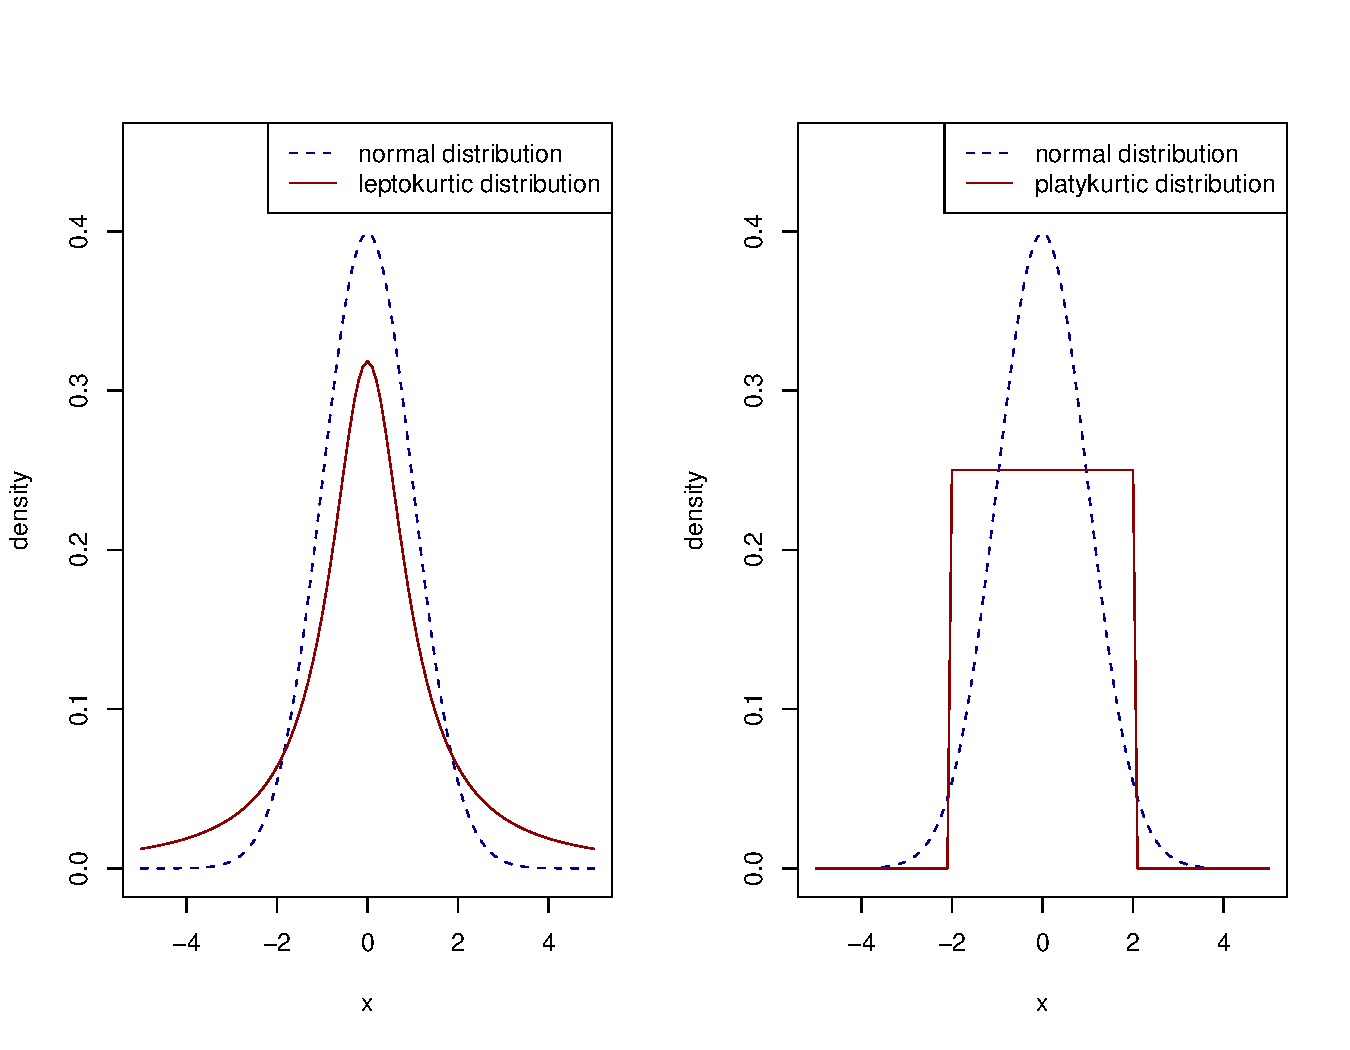
\includegraphics[scale=0.55]{2_kurtosis}
  \end{center}
\end{frame}


\livelloA{Box plot}

\begin{frame}
  \vspace*{.35cm}
  The box-and-whisker diagram or box-and-whisker plot or, simply, the \textbf{box plot} is a convenient way of graphically depicting a distribution of numerical data. The popularity of the box plot (or boxplot) has grown with the implementation in statistical software. The plot is easy to draw and read. \\
  \vspace*{.35cm}
  A box plot shows three fundamental characteristics of a statistical distribution:\\
  \vspace*{.35cm}
  \begin{itemize}
    \item \textbf{the data spread or variability}, with respect of mean and/or median;
    \item \textbf{the skewness};
    \item \textbf{the presence of outliers}.
  \end{itemize}
\end{frame}

\begin{frame}
  \setlength{\unitlength}{.5cm}
  \begin{picture}(50,10)
    \put(3,1){\shortstack{lowest adjacent value}}
    \put(2.75,.75){\framebox(6.75,1.75){}}
    \put(15,1){\shortstack{upper adjacent value}}
    \put(14.75,0.75){\framebox(6.75,1.75){}}
    \put(5.625,2.5){\vector(0,1){1}}
    \put(17.625,2.5){\vector(0,1){1}}
    \put(5.625,3.75){\line(0,1){0.5}}
    \put(17.625,3.75){\line(0,1){0.5}}
    \put(5.625,4){\line(1,0){2}}
    \put(17.625,4){\line(-1,0){4}}
    \put(7.625,4){\line(0,1){1}}
    \put(7.625,4){\line(0,-1){1}}
    \put(13.625,4){\line(0,1){1}}
    \put(13.625,4){\line(0,-1){1}}
    \put(7.625,3){\line(1,0){4}}
    \put(7.625,5){\line(1,0){4}}
    \put(13.625,3){\line(-1,0){2}}
    \put(13.625,5){\line(-1,0){2}}
    \put(10,5){\line(0,-1){2}}
    \put(7.4,5.4){Q1}
    \put(9.5,5.4){Q2=M}
    \put(13,5.4){Q3}
    \put(2,4){\circle*{.25}}
    \put(3.5,4){\circle*{.25}}
    \put(19,4){\circle*{.25}}
    \put(19,5.5){\vector(0,-1){1}}
    \put(18,6){\shortstack{outlier}}
    %\put(16.75,5.75){\framebox(5.75,1.75){}}
    \put(7.4,6.2){$\overbrace{\hspace*{3.2cm}}^{\Delta Q}$}
  \end{picture}
  \begin{small}
    \vspace*{.25cm}
    The \textbf{vertical line} within the box is the \textbf{median}.\\
    \vspace*{.25cm}
    The \textbf{two external vertical lines} that delimit the box are the first ($Q_1$) and the third ($Q_3$) quartiles.
  \end{small}
\end{frame}

\begin{frame}
  \begin{small}
    \vspace*{.35cm}
    The difference between the third and the first quartiles is called \textbf{interquartile range}. It provides a measure of dispersion of the distribution. By definition, the 50\% of observations are included in the interquartile range.\\
    \vspace*{.35cm}
    A small interquartile range means that the 50\% of observed values is close to the median. The size of the interquartile range increases when data dispersion (variability) increases.\\
    \vspace*{.35cm}
    The boxplot provides also information about the shape of the distribution (skewness): if the distance of Q1 from the median differs from the distance of Q3 from the median then the distribution is asymmetric.\\
    \vspace*{.35cm}
    The lines that start from the box borders and stop with a short vertical line are the so called ``whiskers''. The limits given by two whiskers define the ``non-outlier'' range. Any data not included between the whiskers shall be marked as an outlier with a dot.\\
  \end{small}
\end{frame}


% \begin{frame}
%   \begin{footnotesize}
%     \vspace*{.15cm}
%     Naming \textbf{\boldmath{$ r $} the interquartile range}:\\
%     \vspace*{.15cm}
%     $$ r = Q3 - Q1 $$
%     the following quantities can be defined:
%     \vspace*{.15cm}
%     \begin{itemize}
%       \item the \textbf{lower adjacent value (LAV)}: the lowest value still within $1.5 \cdot r$ of the lower quartile:
%         \vspace*{.15cm}
%         $$ \mbox{SO} \geq Q1 - 1.5 r $$
%       \vspace*{.15cm}
%       \item the \textbf{upper adjacent value (UAV)}: the highest value still within $1.5 \cdot r$ of the upper quartile:
%         \vspace*{.15cm}
%         $$ \mbox{LO} \leq Q3 + 1.5r $$
%     \end{itemize}
%     The value 1.5, proposed by Tukey, doesn't have any specific property or meaning. As Tukey said, it has been chosen by his ``experience'', using it statistical ``common sense''.
%   \end{footnotesize}
% \end{frame}
%
% \begin{frame}
%   \vspace*{.35cm}
%   If the smallest or the highest observed values are contained between LAV and UAV then the corresponding whisker will respectively represent the smallest or the highest value.\\
%   \vspace*{.35cm}
%   Values inside the limits (LAV and UAV) can be considered in the standard.\\
%   \vspace*{.35cm}
%   Values outside the limits (LAV and UAV) are defined \textbf{outliers}. In the boxplot they are plotted individually because they are considered anomalous respect to the remaining data of distribution.\\
%   \vspace*{.35cm}
%   Values outside 3 times the interquartile range are \textbf{extreme values} and must be further investigated, to exclude measurement or transcription mistakes.\\
% \end{frame}
%
% \begin{frame}
%   \vspace*{.25cm}
%   The LAV and UAV values, with their distance from quartiles, provide information about data variability and distribution shape.\\
%   \vspace*{.3cm}
%   In the case of a \textbf{gaussian distribution} distances between each quartile and the median are equal. In the same way, also the two whiskers have the same length. \\
%   \vspace*{.3cm}
%   In a normal distribution, whiskers have a distance from the median ($ med $) that is 2.69796 times the standard deviation ($\sigma$).\\
%   \vspace*{.3cm}
%   This range includes a 99.3\% of observations. Outliers are:
%   \vspace*{.25cm}
%   $$ med \pm 2.7 \sigma $$
% \end{frame}
%
% \begin{frame}
%   \begin{center}
%     \includegraphics[scale=1.1]{1_81.png}
%   \end{center}
% \end{frame}



\livelloA{Correlation}

\begin{frame}
  \vspace*{.3cm}
  Statistical indices proposed until now work all on a single variable.\\
  \vspace*{.4cm}
  Given two or more variables, the type and the intensity of the relationship between variables can be analyzed.\\
  \vspace*{.4cm}
  The classical scatterplot (or xyplot) is the most common plot type to show the relationship between two variables.\\
  \vspace*{.4cm}
  Like all graphic tools, it doesn't provide an exhaustive description but it gives hints about the analyzed phenomenon.\\
  \vspace*{.4cm}
  \textbf{If a relationship between variables exists then the scatterplot must show a tendency of the values in variable in the y-axis to vary along with the values in variable in the x-axis.}
\end{frame}

\begin{frame}
  \begin{figure}
    \centering
    \includegraphics[scale=0.4]{1_69.png}
  \end{figure}
  \vspace*{.2cm}
  The plot shows that there is not a relationship between variables or, in other words, it exists a random relationship.
\end{frame}

\begin{frame}
  \begin{floatingfigure}[l]{6.5cm}
    \includegraphics[scale=0.3]{1_70a.png}\\
  \end{floatingfigure}
  \vspace*{.5cm}
  Plots show a relationship between variables.\\
  \begin{floatingfigure}[r]{6.5cm}
    \includegraphics[scale=0.3]{1_70b.png}\\
  \end{floatingfigure}
  \vspace*{1.5cm}
  \hspace*{.2cm}\\
  \hspace*{.2cm}\\
  \hspace*{.2cm}\\
  \hspace*{.2cm}\\
  \hspace*{.2cm}\\
  In both cases the relationship is positive. When x increases also y increases, on average.
\end{frame}

\begin{frame}
  \begin{figure}
    \centering
    \includegraphics[scale=0.35]{1_71.png}
  \end{figure}
  \vspace*{.2cm}
  A \textbf{matrix plot} draws more scatterplots in only one display. It is useful to search for possible relationships between a \textbf{set of variables}.
\end{frame}

\begin{frame}
  \vspace*{.25cm}
  When a \textbf{linear relationship} between two variables exists, then the index that highlights this relationship is the \textbf{covariance} index.\\
  \vspace*{.2cm}
  $$ Cov_{xy} = \frac{\sum_{i=1}^n{\left( x_i-\overline{x}\right)\left( y_i-\overline{y}\right)}}{n-1}  $$\\
  \vspace*{.4cm}
  The covariance can assume:
  \begin{itemize}
    \item \textbf{positive} values, when an increasing linear relationship exists between the two variables;
    \item \textbf{negative} values, when a decreasing linear relationship exists between the two variables;
    \item close to \textbf{zero} values, when a linear relationship doesn't exist between the two variables.
  \end{itemize}
\end{frame}

\begin{frame}
  \begin{figure}
    \centering
    \includegraphics[scale=0.35]{3_quadranti}
    \label{fig:quadranti}
  \end{figure}
\end{frame}

\begin{frame}
  \begin{figure}
    \centering
    \includegraphics[scale=0.35]{3_correl}
    \label{fig:correl}
  \end{figure}
\end{frame}

\begin{frame}
  \begin{itemize}
    \item The graph of Page ~\pageref{fig:quadranti} recalls that the product between x and y is:
      \begin{itemize}
        \item a positive number if x and y are both positive\\ (first quarter, top right);
        \item a negative number if x is negative and y is positive\\ (second quarter, top left);
        \item a positive number if x and y are both negative\\ (third quartrer, bottom left);
        \item a negative number if x is positive and y is negative\\ (quarto quadrante, bottom right).
      \end{itemize}
    \vspace{0.5cm}
    \item The graphs of Page~\pageref{fig:correl} show a state in which:
      \begin{itemize}
        \item there is no correlation between x and y;
        \item there is positive correlation between x and y;
        \item there is negative correlation between x and y.
      \end{itemize}
  \end{itemize}
\end{frame}


\begin{frame}
  \vspace*{.1cm}
  The following inequality can be demonstrated about the covariance:\\
  \vspace*{.25cm}
  $$ -s_x s_y \leq \frac{\sum_{i=1}^n{\left( x_i-\overline{x}\right)\left( y_i-\overline{y}\right)}}{n-1} \leq s_xs_y $$\\
  \vspace*{.25cm}
  As a consequence, the \textbf{correlation index} may be used as a standardized covariance:\\
  \vspace*{.25cm}
  $$ Cor_{xy} = \frac{Cov_{xy}}{s_xs_y} $$\\
  \vspace*{.1cm}
  The correlation index may only assume values between -1 and 1:\\
  \vspace*{.25cm}
  $$ -1 \leq Cor_{xy} \leq 1 $$\\
\end{frame}

\begin{frame}
  \vspace*{.45cm}
  \textbf{Notes}.\\
  \begin{itemize}
    \vspace*{.45cm}
    \item Correlation and covariance are indices that measure only linear relationships. Quadratic, cubic, sinusoidal, ... relationships may also exist between two variables.
    \vspace*{.45cm}
    \item The correlation index can only highlight the linear component of a relationship.
    \vspace*{.45cm}
    \item The presence of correlation may not be due to a cause-and-effect relationship between two variables.
  \end{itemize}
\end{frame}


